% Student template

\clearpage

% Returns a default file if not found
\providecommand\dfincludegraphics[2][]{
	\IfFileExists{#2}
	{
		\includegraphics[#1]{#2}
	}
	{
		%\fbox{File not found}
	}
}

\providecommand\studentimages[1]{%
	\checkoddpage

	% Ring
	% \ifoddpage
	% 	\def\ringx{50pt}
	% \else
	% 	\def\ringx{\pagewdith - 50pt}
	% \fi
	\def\ringx{50pt}
	\def\ringy{250pt}
	\def\ringwidth{250pt}
	\def\ringimgwidth{180pt}
	\def\ringoffset{(\ringwidth - \ringimgwidth) / 2}
	\AddToShipoutPictureBG*{
		\AtTextUpperLeft{
			\put(-\ringx + \ringoffset, -\ringy + \ringoffset){
				\dfincludegraphics[keepaspectratio=true, width=\ringimgwidth]{parts/students/figures/#1.jpg}
			}
			\put(-\ringx, -\ringy){
				
\includegraphics[keepaspectratio=true, width=\ringwidth]{ring.png}
			}
		}
	}

	% Frame
	\def\framex{130pt}
	\def\framey{40pt}
	\def\framewidth{180pt}
	\def\frameimgwidth{160pt}
	\def\frameoffset{(\framewidth - \frameimgwidth) / 2}
	\AddToShipoutPictureBG*{
		\AtTextLowerLeft{
			\put(\textwidth - \framex + \frameoffset, \framey + \frameoffset){
				\dfincludegraphics[keepaspectratio=true, width=\frameimgwidth]{parts/students/figures/#1_child.jpg}
			}
			\put(\textwidth - \framex, \framey){
				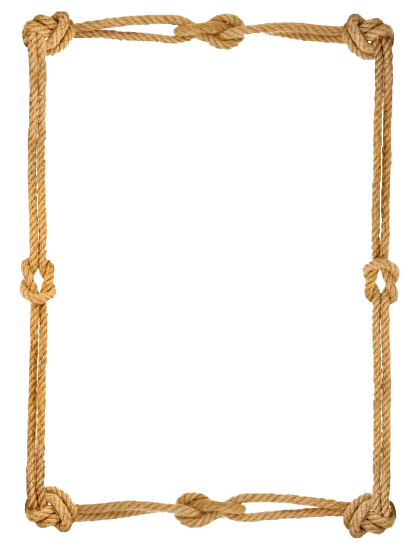
\includegraphics[keepaspectratio=true, width=\framewidth]{rahmen.png}
			}
		}
	}
}

\providecommand\studentprofile[8]{%
	\sectionmark{Steckbrief - #1}

	% Steckbrief Tabelle
	\begin{tikzpicture}[overlay]
		\node[text width=250pt, align=left] at (12, -5) {
			\Large{\begin{tabular}{@{}ll@{}}
					\textbf{Name:}           & #1 \\
					\textbf{Geburtstag:}     & #2 \\
					\textbf{Lieblingsfach:}  & #3 \\
					\textbf{Hobbies:}        & #4 \\
					\textbf{Lieblingsgenre:} & #5 \\
				\end{tabular}}\\~\\
			\textbf{Das werde ich am meisten vermissen:}\\#6\\~\\
			\textbf{Ohne das hätte ich die Oberstufe nicht geschafft:}\\#7\\~\\
			\textbf{Lebensmotto:}\\#8\\~\\
		};
	\end{tikzpicture}
}

\providecommand\studenttable[2]{%
	\vskip 10cm
	\hspace*{-1.2cm}
	\Large{\begin{tabular}{@{}ll@{}}
			\textbf{Erkennungsmerkmale:} & #1 \\
			\textbf{Zukunftspläne:}      & #2 \\
		\end{tabular}}
}

\providecommand\studentcomments[1]{%
	\begin{figure}[H]
		\hspace*{-2.5cm}
\includegraphics[keepaspectratio=true, width=\paperwidth]{mittelwelle.png}
	\end{figure}
}
